
\chapter{Background and Related Work}

\label{ch:background}

\section{Introduction}

This chapter begins with a brief overview of reconfigurable systems in Section~\ref{sec:bg_reconfig}.
The underlying system architecture and the design flow that maps designs to this system are illustrated.
Real-time systems and their typical applications are covered in Section~\ref{sec:bg_realtime}.
Section~\ref{sec:bg_summary} provides a summary.

\section{Reconfigurable Systems}
\label{sec:bg_reconfig}

\subsection{Architecture}

The underlying technology of reconfigurable system is \gls{fpga}.
In order to perform as functional circuits, \glspl{fpga} provide numerous fine-grained resources, namely \glspl{lut} implemented in small \glspl{ram}.
\glspl{lut} implement combinational logic by storing the corresponding truth table and using the logic inputs as the address into the \glspl{lut}.
\glspl{fpga} enable sequential circuits by providing registers along \gls{lut} outputs.
By providing hundreds of thousands of \glspl{lut} and registers, \glspl{fpga} can implement massively parallel circuits.
Modern FPGAs also have coarse-grained resources such as \glspl{clb}, multipliers, \glspl{dsp}, on-chip \glspl{ram}, and even microprocessor cores.
Microprocessor cores can be dedicated hard processor, such as ARM Cortex A9 in Altera \gls{soc}-\gls{fpga}~\cite{alterasoc} and Xilinx Zynq~\cite{xilinxzynq}.
In addition, designers can use the \glspl{lut} to implement soft processors, such as Altera's Nios II~\cite{alteranios2} and Xilinx's MicroBlaze~\cite{xilinxmicroblaze}.

To combine these resources into larger circuits, \glspl{fpga} provide reconfigurable interconnect.
In between each row and column of resources, \glspl{fpga} contain numerous routing tracks, which are wires carrying signals across the chip.
Connection boxes provide programmable connections between resources \gls{io} and routing tracks, while switch boxes provide programmable connections between intersecting routing tracks.
Such programmable connections allow a signal to be routed to any destination on the \gls{fpga} chip.
This architecture is called an island-style fabric as shown in Figure~\ref{fig:bg_islandstyle}.

\begin{figure}[ht]
\begin{center}
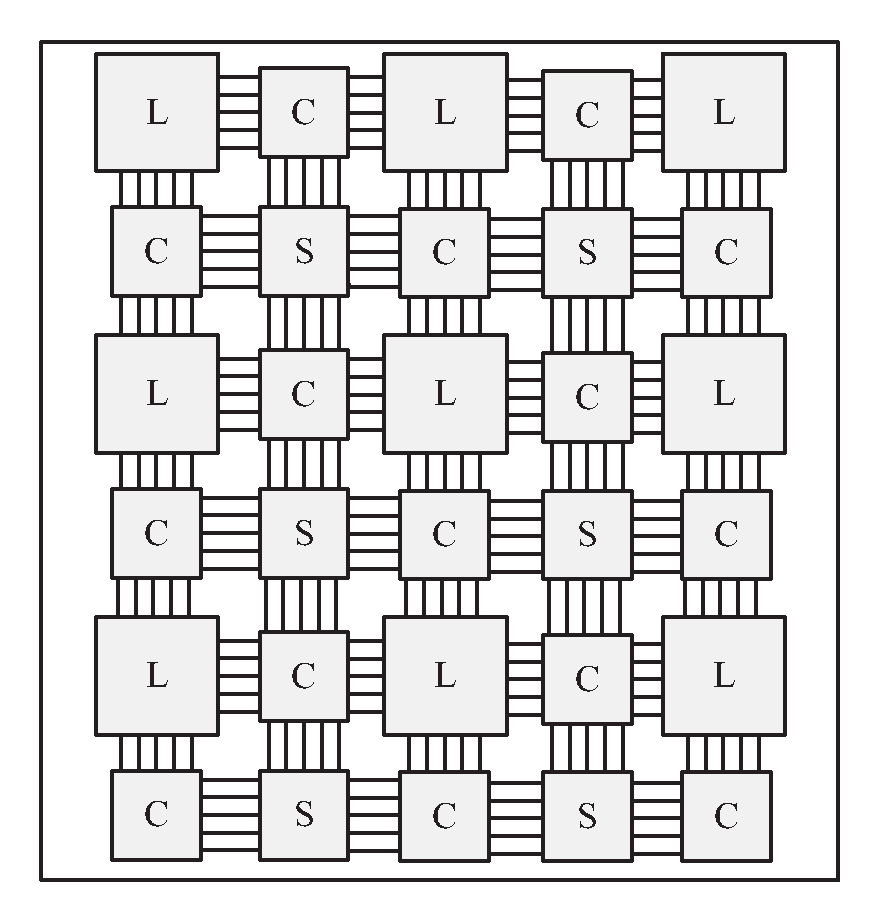
\includegraphics[width=0.5\textwidth]{2_background/figures/islandstyle}
\end{center}
\caption{Island-style FPGA (L: LUTs and coarse-grained resources; C: Connection boxes; S: Switch boxes).}
\label{fig:bg_islandstyle}
\end{figure}

The reconfigurability of ~\glspl{fpga} leads to an unique feature which allows circuitry to be selectively updated on the fly, without disturbing the execution of the remaining system.
This technique is referred to as run-time reconfiguration or dynamic reconfiguration.
%Many dynamically reconfigurable architectures ~\cite{trimberger97,fujii99} have been proposed.
In~\cite{trimberger97}, a time-multiplexed \gls{fpga} is proposed.
The \gls{fpga} can store eight configurations and switch between each of them in 30ns.
The ability of changing the entire configuration of the \gls{fpga} in a single cycle allows the \gls{fpga} to emulate a single large design, or to share the resource to run several independent designs.
However, they express concern about the power consumption when the device is reconfigured frequently, though the device has not yet been fabricated and tested.
Another dynamically reconfigurable architecture is proposed in~\cite{fujii99}.
To accommodate eight configurations for multi-context, 35\% of area penalty is incurred.
Although the idea of time-multiplexing is intriguing, the above mentioned architectures do not identify any killer application which can benefit from this ability.

\glspl{fpga} are used to create specialised circuits for tailored toward specific applications, and have the potential to provide significant performance improvement compared to general-purpose microprocessors.
On the other hand, general-purpose microprocessors are easier to program and have higher binary compatibility among different processor models.
Tightly-coupled reconfigurable coprocessors are proposed.
Garp~\cite{hauser97} has an \gls{fpga} located on the same die as the processor.
While the \gls{fpga} provides coarse-grained acceleration such as pipelined and parallelised loops, the main processor takes care of all other computations.
The programmability of the \gls{fpga} remains a challenge when users have to manually specify the configuration of logic block and connections.
Chimaera~\cite{ye00} targets a more fine-grained acceleration by collapsing performance-critical instructions into specific operations for an on-chip reconfigurable unit.
The data-path of the reconfigurable unit is tailored for those specific operations, thus offers performance improvement.

\glspl{fpga} have also been employed in \gls{hpc} serving as accelerators in computing clusters.
There exists a number of reconfigurable architectures which target compute-intensive applications.
Convey HC-2 Computer~\cite{conveyhc2} integrates an FPGA-based reconfigurable co-processor with Intel-based x86 host.
The co-processor's FPGAs execute compute-intensive operations which take a large component of an application's run-time.
The HC-2 system has a memory subsystem and crossbar which provide a highly parallel and high bandwidth (80 GB/s) connections between the FPGAs and the corresponding physical memory.
It also employs a scatter-gather dual inline memory modules (SG-DIMMs) to increase performance of random memory access.
Meanwhile, Maxeler Technologies develop a series of reconfigurable systems which consist of Intel-based x86 host and FPGA-based data-flow engines~\cite{maxeler}.
Their MPC-C500 machine can deliver over 400 GFLOPS computation speed and over 35GB/s of bandwidth to external physical memory.

To leverage the advantages of \gls{fpga}s for hardware acceleration, Chow et al.~\cite{chow11} proposed a mixed precision methodology.
%The work made an assumption that the data-path is short so that both the reduced precision and high precision implementations can fit in a single \gls{fpga}.
%They also assume that the communication between the reduced-precision data-path and the high-precision data-path is completed via a crossbar, thus the overhead is negligible. 
%For complicated applications where the level of parallelism is limited by \gls{fpga} resource, their approach is not applicable.
%On the other hand, they are not applicable for complicated applications when the level of parallelism is limited.
There are studies on bit-width optimisation which uses minimum precision in a data-path given a required output accuracy.
Examples include interval arithmetic~\cite{fang03}, affine arithmetic~\cite{lee05,osborne07} and polynomial algebraic approach~\cite{boland10}.
However, a reduction of precision in any stage within a data-path will result in a loss in output accuracy which is uncorrectable.
These studies require the use of accuracy models to relate output accuracy with the precisions of data-path.
%In contrast to these work, we focus on using run-time reconfiguration to derive an automatic way so as to find an optimal precision.
%Our work is different from these work by deriving an automatic way to find an optimal precision using run-time reconfiguration.

\subsection{Design Flow}

To enable implementation of applications on \glspl{fpga}, \gls{fpga} tools generally support a design flow as shown in Figure~\ref{fig:bg_flow}.
Firstly, \textit{synthesis} takes source files written at \gls{rtl}, typically written in \gls{hdl}, and converts them to design implementation in terms of logic gates.
Secondly, \textit{technology mapping} converts all logic gates into device resources such as \glspl{lut}, \glspl{dsp} and block \glspl{ram}.
Thirdly, \textit{placement} maps each technology-mapped component onto physical locations of the chip.
Finally, \textit{routing} programs the interconnect to implement all connections in the circuit and generates a bit-stream which is downloaded to configure the target \gls{fpga}.

\begin{figure}[ht]
\begin{center}
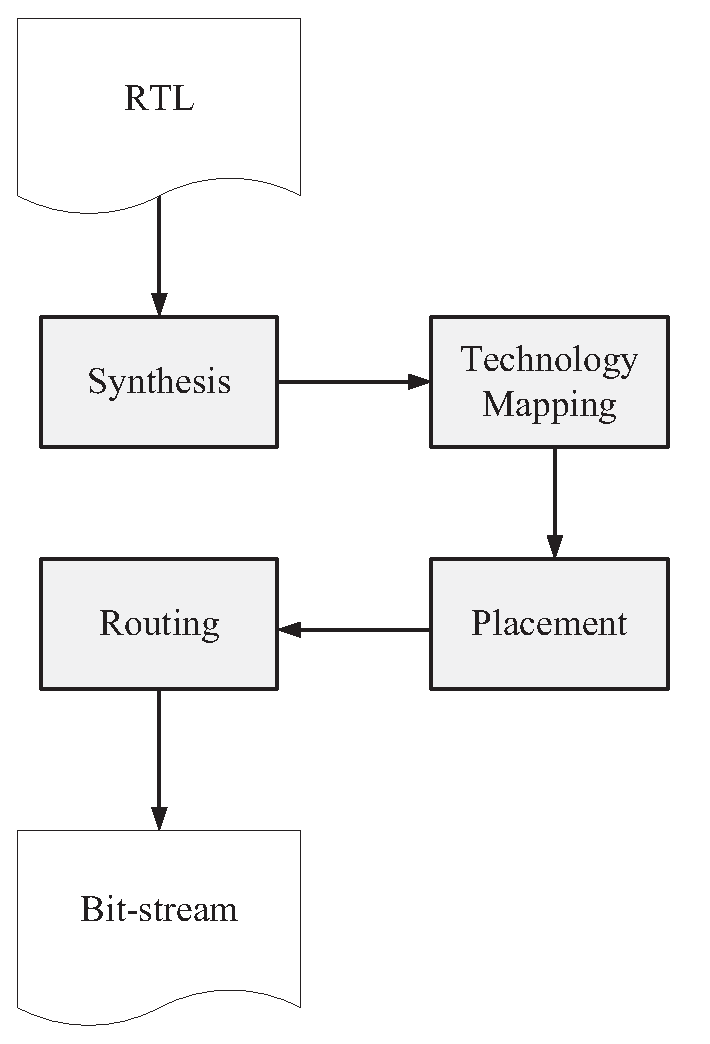
\includegraphics[width=0.8\textwidth]{2_background/figures/flow}
\end{center}
\caption{Design flow of FPGAs.}
\label{fig:bg_flow}
\end{figure}

There are two major programming models for \glspl{fpga}.
The most common model manually converts the code into a semantically equivalent \gls{rtl} circuit, which designers typically specify using \glspl{hdl} such as VHDL and Verilog.
Designing \gls{rtl} circuits is time consuming.
Designers must specify the entire structure of the data-path, define control for components, and manage data movement from inputs to outputs which involve devices such as DDR memory, PCI Express bus, ethernet, and so on.
Such complexity leads researchers to work on \gls{hls} tools which synthesise algorithmic descriptions from high-level languages, such as SystemC and Ansi C/C++, to  \gls{rtl} circuits.
Commercial \gls{hls} tools become increasingly common.
Example includes Xilinx's Vivado HLS~\cite{xilinxvivado}, Impulse Accelerated Technologies' Impulse C~\cite{impulsec}, Calypto's Catapult C~\cite{catapultc}, Mentor Graphics' Handel-C~\cite{handelc}, IBM's Lime~\cite{lime}, Bluespec~\cite{bluespec}, OpenSPL~\cite{openspl,maxcompiler}, OpenCL in Altera \glspl{fpga}~\cite{alteraopencl}, and MathWorks' Simulink (via HDL Coder~\cite{hdlcoder}, DSP Builder~\cite{alteradspbuilder} and System Generator~\cite{xilinxsysgen}).
Open-source tools such as LegUp~\cite{legup} are also gaining researchers' attention.

%\todo[inline]{ HW/SW co-design approach~\cite{shenoy01,noguera01}.}
As mentioned earlier, tightly-coupled reconfigurable coprocessors are integrated to \glspl{cpu}, to achieve higher performance.
Hardware-software co-design approaches are proposed to exploit these architectures.
In~\cite{li00}, system-level applications specified in C are partitioned onto \gls{cpu} and \gls{fpga}
Instruction-level parallelism is extracted for hardware acceleration, and the configuration time of \gls{fpga} is considered.
In~\cite{li02}, a multi-objective approach is developed which assign multi-rate and real-time tasks to systems consisting of \glspl{fpga} and processors.
The partitioning algorithm is able to optimise schedule length and power consumption simultaneously.
As the run-time overhead of reconfiguring \glspl{fpga} is significant, early partial reconfiguration and incremental reconfiguration techniques are proposed in~\cite{jeong00}.
The reconfiguration time is hidden in the slack interval when the software part is executing.
The approaches mentioned above assume the \gls{fpga} is too small to fit in the entire application, thus run-time reconfiguration is exploited to utilise the \gls{fpga} as much as possible.
However, \glspl{fpga} nowadays have plenty of logic resources, and even multiple \glspl{fpga} work together for an application.
The application can be extensively parallelised with deep pipelines, and makes use of coarse-grain resources such as \gls{dsp} and floating-point units~\cite{alteraarria10} for arithmetic operations in custom bit-width.
New approaches are needed for the latest architectures.

Heterogeneous computing is becoming more popular, many \gls{hpc} systems use a combination of off-the-shelf devices including \glspl{cpu} and \glspl{fpga}.
OpenSPL and OpenCL are two standards which have been proposed to provide a framework for writing programs that execute across \glspl{fpga}, \glspl{cpu} and \glspl{gpu}.
Figure~\ref{fig:openspl} illustrates the conceptual design flow of \gls{fpga} with OpenSPL and OpenCL.
Both OpenSPL~\cite{openspl} and OpenCL include software-like programming language for developing kernel (functions that execute on hardware devices) as well as application programming interfaces that allow kernels communicate with software executable running on micro-processors.
OpenSPL, which stands for Open Spatial Programming Language, is a programming language focusing on data-flow computing.
Maxeler Technologies' MaxCompiler~\cite{maxcompiler} is a commercial tool which supports OpenSPL and a series of reconfigurable \gls{hpc} systems.
Traditionally, designers targeting different \glspl{fpga} must make significant board-specific changes to RTL circuits which are described at low-level.
OpenSPL simplifies the effort of customising an \gls{fpga} application for a specific model of \gls{fpga} by automatically generating interfaces such as buses between \glspl{cpu} and \glspl{fpga}, as well as controller for external memory.
In addition, OpenSPL provides functional level simulation which reduces the debugging effort on \gls{rtl}-level code simulation.
On the other hand, OpenCL, which stands for Open Computing Language, is being promoted by Altera to target software developers who are new to \glspl{fpga}.
As the requirement of hardware knowledge is low compared to traditional \gls{hdl} development, OpenCL enables designers focus on high-level algorithm and software system design.

\begin{figure}[ht]
\begin{center}
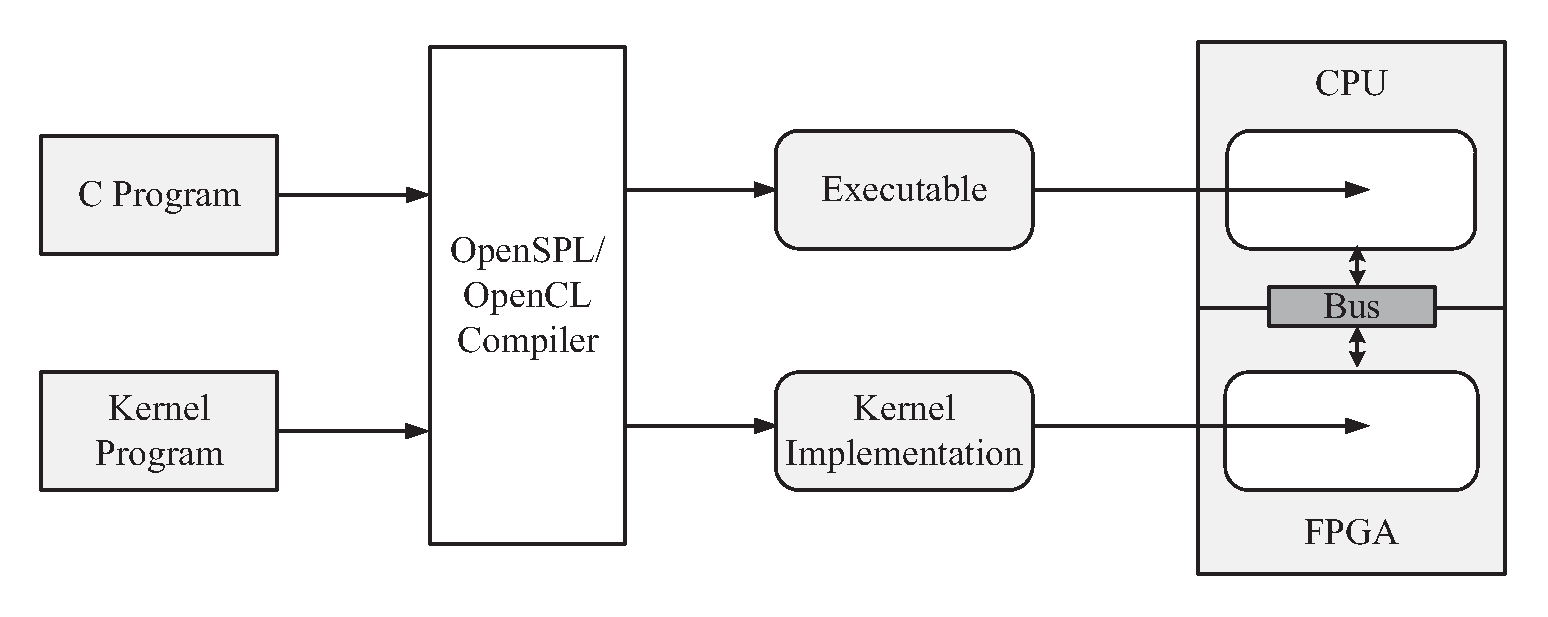
\includegraphics[width=0.95\textwidth]{2_background/figures/openspl}
\end{center}
\caption{Design flow of FPGA with OpenSPL and OpenCL.}
\label{fig:openspl}
\end{figure}

MathWorks promote \gls{hls} with a model-based design flow~\cite{mathworks,sharma09}.
As shown in Figure~\ref{fig:hdlcoder}, designers first simulate and verify operations in the Simulink development environment, then \gls{fpga} \gls{ip} cores are generated from the Simulink models using HDL Coder, while software executables for ARM processor are compiled using Embedded Coder.
The design flow also includes various board-support-packages which generate device-specific interfaces automatically.

\begin{figure}[ht]
\begin{center}
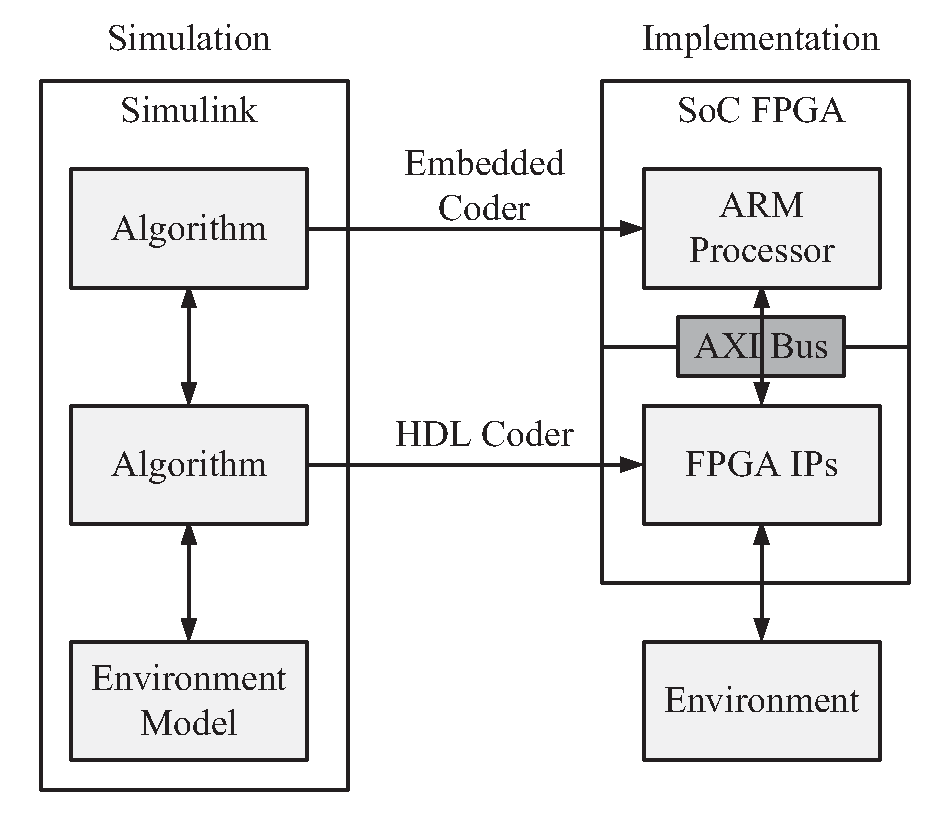
\includegraphics[width=0.7\textwidth]{2_background/figures/hdlcoder}
\end{center}
\caption{Model-based design flow.}
\label{fig:hdlcoder}
\end{figure}

Even though \gls{hls} tools ease the development effort of building parallelised applications that fully take advantage of \gls{fpga},
designers still suffer from long synthesis time which makes design space exploration very inefficient.
Traditional software techniques relying on rapid recompilation are no longer feasible.
The design space exploration of reconfigurable designs requires substantial effort from users who have to analyse the application, create models and benchmarks, and subsequently use them to evaluate the design.
Sometimes such an approach is infeasible as numerical properties cannot result in a closed-form analytical model.
One can proceed with automated optimisation based on an exhaustive search through design parameters, yet even automation of design space exploration is problematic because of the large number of evaluations needed.
In dealing with large design space, an optimisation approach~\cite{kurek13arc} is developed based on Efficient Global Optimisation (EGO)~\cite{jones98}.
It has a surrogate model consisting of both a Gaussian process regressor~\cite{rasmussen06} and a Support Vector Machine (SVM) classifier~\cite{basudhar12}.
By using the surrogate model, the algorithm allows for automated design space exploration.
The classification mechanism employed in the optimisation approach allows for constrained optimisation and it is particularly designed to cope with reconfigurable designs parameter tuning. 
This work is extended in~\cite{kurek14fccm} to offer automatic and calibration free optimisation.

\subsection{Domain Specific Languages}
At present, \glspl{fpga} are mainly programmed in \gls{rtl} using Verilog or VHDL. 
The long development times and requirement for low-level, hardware-centric design expertise have served as a historical barrier for programmers and software engineers. 
\gls{rtl} design is error prone and non-portable.
\glspl{dsl} or \glspl{dcl} are being promoted to increase programmer productivity and code quality.
\glspl{dsl} allow application to be described using abstractions that are closer to a problem domain. 

GraphGen~\cite{nurvitadhi14} is a vertex-centric framework that targets \gls{fpga} for graph computations.
The framework accepts a vertex-centric graph specification and automatically compiles it onto an application-specific synthesised graph processor.
The graph processor is customisable by user-defined graph instructions.
There is also a special-purpose memory subsystem for graph computations.
In the area of packet parsing, G~\cite{brebner09} and PP~\cite{attig11} are high-level programming languages which can be compiled to produce high-speed \gls{fpga}-based packet parsers.
%Model-based design~\cite{sharma09} is employed by MathWorks to reduce the design and verification effort of FPGAs for automotive applications.

\section{Real-time Systems}
\label{sec:bg_realtime}

%A real-time system is one which must process information and produce a response within a specified time. %otherwise severe consequences, including failure, can result.
A system is defined as being real-time if it is required to respond to an input stimulus within a finite and specified time interval.
The stimulus could either be an event at the interface to the system or an internal signal.
The correctness of a real-time system is based on both the correctness of the outputs and their timeliness.
However, the system does not have to be fast.
A hard real-time system should guarantee a response to events within a timing bound which is normally referred to as a \textit{deadline}.
Missing an operation deadline can lead to catastrophic effects such as a total system failure. 
Soft real-time system is a loosen form where exact response time is not critical, but missing an operation deadline can cause degraded quality of service.
%Uncomfortably long response times cause degraded quality of service but the system still functions even if deadlines are sometimes not met.

%\pagebreak
In summary, real-time systems must have the following properties to support critical applications~\cite{buttazzo11}:
\begin{itemize}
\item Timeliness: Output values are produced before the deadlines.
\item Robustness: The system should work when subject to a peak load.
\item Predictability: The system behaviour is known before it is put into operation.
%\todo[inline]{Before the deadline or right at the deadline?}
%\item Testability: the system can be tested whether it can meet all deadlines.
%\item Fault tolerance: Failures of software and hardware should not cause the system to crash.
%\item Maintainability: The architecture of a real-time system should be designed to ensure that system modifications are easy to perform.
\end{itemize}

This thesis focuses on accelerating high performance real-time applications using reconfigurable systems. 
To ensure the implementations have the above-mentioned properties, we will discuss performance models and measurement-based approaches which analyse the worst case timing behaviour.
In the following chapters, we will apply reconfigurable technologies to three important real-time applications and shows the benefits of reconfigurable systems to real-time applications.

\subsection{Real-time Applications}

\subsubsection{A. Proximity Query for Image-guided Surgery}

Advanced surgical robots support image guidance and force-based haptic feedback for effective navigation of surgical instruments. 
Such image-guided robots rely on real-time computing the intersection or the closest point-pair
between two objects in three-dimensional space; 
this computation is known as \gls{pq}.

\gls{pq} has been widely studied in areas such as robot motion planning, haptics rendering, virtual prototyping, computer graphics, and animation~\cite{gilbert90}.
Robot motion planning is particularly demanding for the real-time performance of \gls{pq}~\cite{chakraborty08}. 
In the past decade, \gls{pq} has also been used as a key task for active constraints~\cite{kwok10} and virtual fixtures~\cite{li07}, which are collaborative control strategies mostly applied in image-guided surgical robotics. 
The clinical potential of this control strategy has been demonstrated by imposing haptic feedback~\cite{constantinescu05} on instrument manipulation based on imaging data~\cite{jakopec03}.
This haptic feedback provides the operator with kinaesthetic perception for sensing positions, velocities, forces, constraints and inertia associated with direct maneuvering of surgical
instrument within the target anatomy.

Fast and efficient \gls{pq} is a pre-requisite for effective navigation through access routes to the target anatomy~\cite{kwok10}.
Haptic guidance, rendered based on imaging data, can enable a distinct awareness of the position of the surgical device relative to the target anatomy so as to prevent the operator from feeling disoriented within the surrounding organs. 
Such disorientation could potentially cause unnoticed major organ damage. 
Haptic guidance is particularly important during soft tissue surgery, which involves large-scale and rapid tissue deformations. 
A high update frequency above 1~kHz is required to maintain smooth and steady manipulation guidance. 
Due to its intrinsic complexity and this real-time requirement, \gls{pq} is computationally challenging.
Various approaches have been proposed to achieve the required update rate~\cite{benallegue09,chakraborty08}, 
with objects represented in specific formats such as spheres, torus or convex surfaces.
The only attempts that apply \gls{pq} to haptic rendering, while considering explicitly the interaction of the body with the surrounding anatomical regions, involve modelling the anatomical pathway or the robotic device as a tubular structure~\cite{li07,kwok13}.
The computation burden is increased by the need to compute the placement of anatomical model relative to the robot whose shape is represented by more than~1~million~points.

%\subsection{Geometric Representation for \gls{pq}}
Fig.~\ref{fig:pqa} illustrates two objects acting as inputs to \gls{pq}. 
The tubular object is bounded by a series of contours $C_j$ $\forall j \in [1,...,N_C]$, each of which is outlined by a set of contour points. 
This object can be either a luminal anatomy or a robotic endoscope or catheter. 
Inside the tubular object, the mesh comprises points which represent the morphological structure of either the robot or the target anatomy in complex shape. 
Essentially \gls{pq} computes $\delta_j$, which describes how much the mesh deviates beyond the volumetric pathway bounded along the contours.

\begin{figure}[ht]
\begin{center}
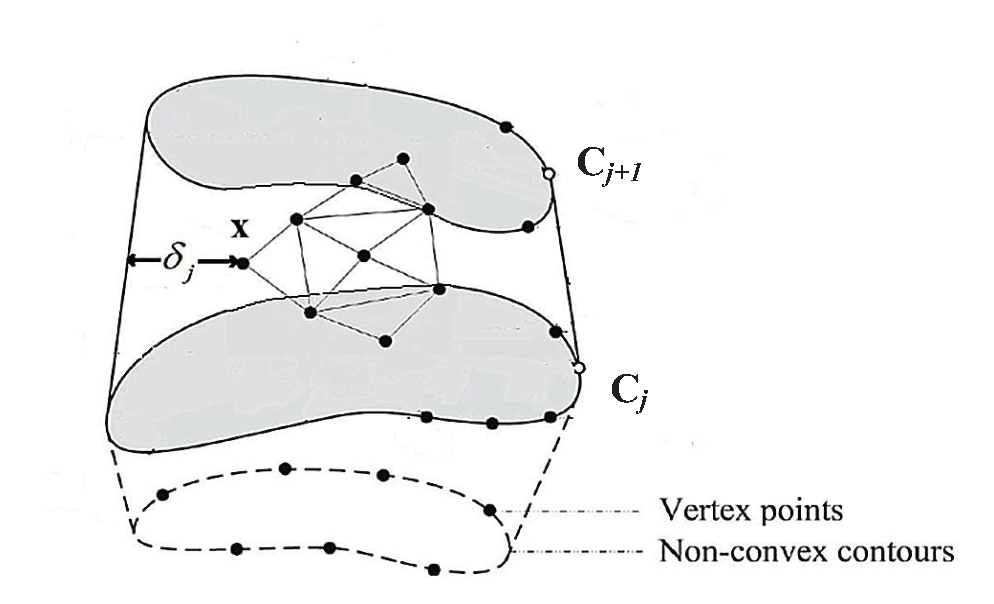
\includegraphics[width=0.65\textwidth]{2_background/figures/pqa}
\end{center}
\caption[Sets of points aligned on a series of contours and a set of points located on an arbitrary form of mesh.]{Sets of points aligned on a series of contours and a set of points located on an arbitrary form of mesh.}
\label{fig:pqa}
\end{figure}

\setcounter{subfigure}{0}
\begin{figure}[t!]
\centering
\subfigure[]{
	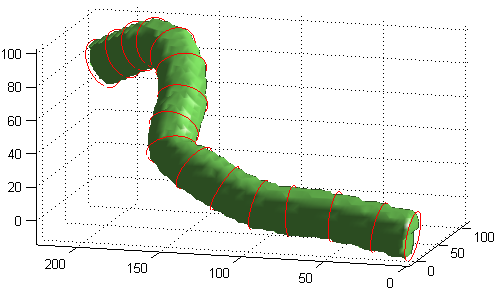
\includegraphics[width=0.7\textwidth]{3_precision/figures/tube1}
	\label{fig:tube1}
}
\subfigure[]{
	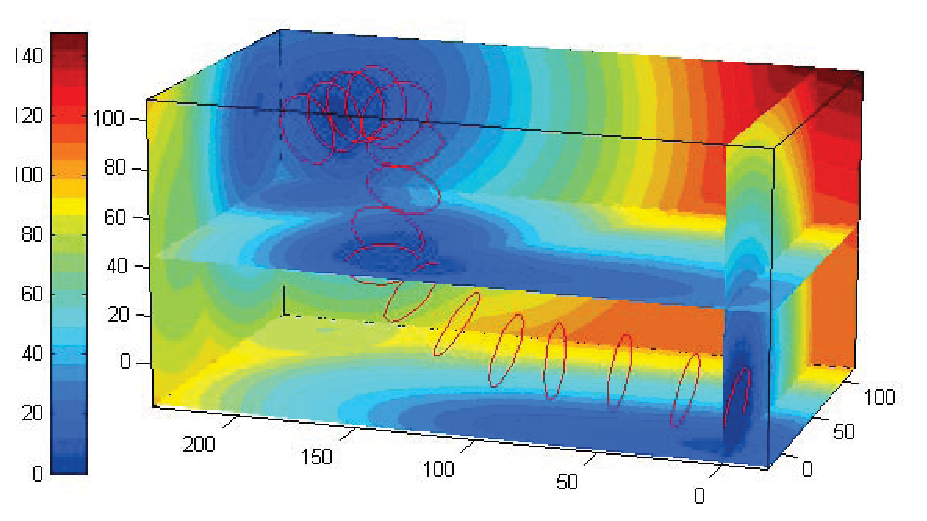
\includegraphics[width=0.7\textwidth]{3_precision/figures/tube2}
	\label{fig:tube2}
}
\caption[(a) A virtual tube bounded by a series of contour denotes the configuration of an endoscope;
(b) The corresponding three-dimensional distance map in grids of 86x48x43.]{(a) A virtual tube (in green) bounded by a series of contour (in red) denotes the configuration of an endoscope;
(b) The corresponding three-dimensional distance map in grids of 86x48x43.}
\label{fig:tube}
\end{figure}

As shown in Fig.~\ref{fig:tube1}, a series of circular contours fitted along a part of an endoscope, which passes through the rectum up to the sigmoid colon. 
These contours form a constraint pathway. 
Fig.~\ref{fig:tube2} shows a distance map in three-dimensional space with 177k grid points. 
Distance from every grid point to the endoscope is computed by \gls{pq}. 
The warmer colour, the further the point is located beyond the endoscope.
%Each contour is denoted by $C_j$, $\forall j \in [1,...,N_C]$.
%A single segment $\Omega_j$ comprises two adjacent contours $C_j$ and $C_{j+1}$.
%$P_j$ is the centre of the contour $C_j$.
%$M_j$ is the tangent of centre line of contour $C_j$.
%$^j\omega_i=[^j\omega_{xi},^j\omega_{yi},^j\omega_{zi}]^T, (i=1,...,W)$ are the contour points,
%where $W$ is the number of points outlining each contour.

%\subsection{Hardware Acceleration for \gls{pq}}
There has been previous work on hardware acceleration of board-phase \gls{pq}, which involves detecting collisions between primitive objects, e.g. spheres~\cite{benallegue09} or boxes~\cite{zhang07}. 
Such an object can be a bounding volume tightly containing a union of multiple complex-shaped objects. 
On \glspl{fpga}, the most relevant work is covered by Chow el at.~\cite{chow11}.
On the other hand, narrow-phase \gls{pq}, which computes the shortest distance or penetration depth between polyhedra, such as GJK~\cite{gilbert88}, V-Clip~\cite{mirtich98} and Lin-Canny~\cite{lin91}, are difficult to be accelerated by hardware due to algorithmic complexity. 
There is, thus far, no attempt of using \gls{fpga}. 
In addition, such approaches are restricted to the object represented in convex polyhedra. 
To this end, a \gls{pq} approach for complex-morphology object~\cite{kwok13} is proposed but how it can be incorporated with \gls{fpga} is not elaborated.
%and also demonstrate how it can be well-incorporated with \gls{fpga}. 

%As mentioned above, fast and efficient \gls{pq} is a pre-requisite for effective navigation through access routes to the target anatomy~\cite{kwok10}.
%This haptic guidance, rendered based on imaging data, can enable a distinct awareness of the position of the surgical device relative to the target anatomy so as to prevent the operator from feeling disoriented within the surrounding organs. 
%Such disorientation could potentially cause unnoticed major organ damage. 
%This guidance is particularly important during soft tissue surgery, which involves large-scale and rapid tissue deformations. 
%A high update frequency above 1~kHz is required to maintain smooth and steady manipulation guidance. 
%Due to its intrinsic complexity and this real-time requirement, \gls{pq} is computationally challenging.
%Various approaches have been proposed to achieve the required update rate~\cite{benallegue09,chakraborty08}, 
%with objects represented in specific formats such as spheres, torus or convex surfaces.
%The only attempts that apply \gls{pq} to haptic rendering, while considering explicitly the interaction of the body with the surrounding anatomical regions, involve modelling the anatomical pathway or the robotic device as a tubular structure~\cite{li07,kwok13}.
%The computation burden is increased by the need to compute the placement of anatomical model relative to the robot whose shape is represented by more than~1~million~vertices.


\subsubsection{B. SMC Methods for Robotic and Control}
\label{sec:smc}

\gls{smc} methods, also known as particle filter, are a set of a posterior density estimation algorithms that perform inference of unknown quantities of interest from observations~\cite{doucet01}.
The observations arrive sequentially in time and the inference is performed on-line.
\gls{smc} methods are often preferable to Kalman filters and hidden Markov models, as they do not require exact analytical expressions to compute the evolving sequence of posterior distributions.
\gls{smc} methods work well for dynamic systems involving non-linear and non-Gaussian properties, and they can model high-dimensional data using non-linear dynamics and constraints, are parallelisable, and can greatly benefit from hardware acceleration.
\gls{smc} has been studied in various application areas including object tracking~\cite{happe11}, robot localisation~\cite{montemerlo02}, speech recognition~\cite{vermaak02} and air traffic management~\cite{kantas09,eele11}.
For these applications, it is critical that high sampling rates can be handled in real-time.
\gls{smc} methods also have applications in economics and finance~\cite{creal12} where minimising latency is crucial.

\gls{smc} keeps track of a large number of particles, each contains information about how a system would evolve.
The underlying concept is to approximate a sequence of states by a collection of particles.
Each particle is weighted to reflect the quality of an approximation.
The more complex the problem, the larger the number of particles that are needed.
One drawback of \gls{smc} is its long execution times so its practical use is limited.

%\gls{smc} methods estimate the unobserved states of interest based on observations in controlling various agents.
In \gls{smc}, the target posterior density $p(s_t|m_t)$ is represented by a set of particles, where $s_t$ is the state and $m_t$ is the observation at time-step $t$.
A sequential importance resampling algorithm~\cite{gordon93} is used to obtain a weighted set of $N_P$ particles $\{s_t^{(i)},w^{(i)}\}^{N_P}_{i=1}$.
The importance weights $\{w^{(i)}\}^{N_P}_{i=1}$ are approximations to the relative posterior probabilities of the particles such that $\sum^{N_P}_{i=1}w^{(i)}_t = 1$.
This process is described in Algorithm~\ref{algo:smc_bg}.
A more detailed description can be found in~\cite{doucet01}. 

\begin{algorithm}
\caption{\gls{smc} methods.}
\begin{algorithmic}[1]
\FOR {each time-step $t$}
\STATE {$idx1 \gets 0$}
\STATE {Initialisation}
\WHILE {$idx1 \le itl\_outer$}
	\STATE {$idx2 \gets 0$}
	\STATE {$itl\_inner \gets f(idx1)$}
	%3+5\exp(\frac{5*idx1}{itl\_outer})$}
	\FOR {each particle p}
		\WHILE {$idx2 \le itl\_inner$}
			\STATE {Sampling} \label{algo:s}
			%\STATE {\hspace{\algorithmicindent}$\hookrightarrow$ Disturbance realisation}
			%\STATE {\hspace{\algorithmicindent}$\hookrightarrow$ Trajectory planning}
			\STATE {Importance weighting} \label{algo:i}
			%\STATE {\hspace{\algorithmicindent}$\hookrightarrow$ Score calculation}
			%\STATE {\hspace{\algorithmicindent}$\hookrightarrow$ Constraint handling}
			%\STATE {\hspace{\algorithmicindent}$\hookrightarrow$ Weight calculation and normalisation}
			\STATE {$idx2 \gets idx2+1$}
		\ENDWHILE
	\ENDFOR
	\STATE {$idx1 \gets idx1+1$}
	\IF {$idx1 \le itl\_inner$}
		\STATE {Resampling}
	\ENDIF
\ENDWHILE
\STATE {Update}
\ENDFOR
\end{algorithmic}
\label{algo:smc_bg}
\end{algorithm}

\begin{enumerate}
\item \textbf{Initialisation}: Weights $\{w^{(i)}\}^{N_P}_{i=1}$ are set to the same value, e.g. $\frac{1}{N_P}$.
\item \textbf{Sampling}: Next states $\{s_{t+1}^{\prime(i)}\}^{N_P}_{i=1}$ are computed based on the current state $\{s_{t}^{(i)}\}^{N_P}_{i=1}$.
The states can be simulated forward over the prediction horizon for $H$ sampling intervals.
\item \textbf{Importance weighting}: Weight $\{w^{(i)}\}^{N_P}_{i=1}$ is updated based on a score function which accounts for the likelihood of particles fitting the observation.
Within each iteration of $itl\_outer$, the sampling and importance weighting stages are iterated $itl\_inner$ times so that those particles with sustained benefits are assigned higher weights.
$itl\_inner$ increases as a function of $idx1$, because a larger $idx1$ implies that the set of particles reflects a more accurate approximation.
\item \textbf{Resampling}: Particles with small weights are removed and those with large weights are replicated.
This process is repeated for $itl\_outer$ times in a time-step to address the problem of degeneracy~\cite{kitagawa96}.
Without resampling, only a small number of particles will have substantial weights for inference.
\item \textbf{Update}: State $s_{t+1}$ is obtained from the resampled particle set $\{s_{t+1}^{(i)}\}^{N_P}_{i=1}$ via weighted average or more complicated functions.
\end{enumerate}

Table~\ref{tab:parameters} summarises the parameters of the \gls{smc} methods described in Section~\ref{sec:smc}.

\begin{table}
	\setlength{\tabcolsep}{3pt}
	\begin{spacing}{1.0}
	\caption{SMC design parameters. Dynamic: adjustable at run-time; Static: fixed at compile-time.}
	\label{tab:parameters}
	\footnotesize
	\centering
	\smallskip
		\begin{tabular}{c|c|c}
			\hline
			 Parameters & Description & Type\\
			\hline
			\hline
			$itl\_outer$ & Number of iterations of the outer loop & \multirow{4}{*}{Dynamic}\\
			$itl\_inner$ & Number of iterations of the inner loop &\\
			$N_P$ & Number of particles &\\
			$S$ & Scaling factor for standard deviation of noise &\\
			\hline
			$H$ & Prediction horizon & \multirow{2}{*}{Static}\\
			$N_A$ & Number of agents under control &\\
			\hline
		\end{tabular}
		\end{spacing}
\end{table}

%\gls{pf} estimates the state of a system by a sampling-based approximation of the state probability density function. 
%The state of a system in time-step $t$ is denoted by $X_t$. 
%The control and observation are denoted by $U_t$ and $Y_t$ respectively. 
%Three pieces of information about the system are known a-priori: 
%\begin{itemize}
%\item $p(X_0)$ is the probability of the initial state of the system, 
%\item $p(X_t|X_{t-1},U_{t-1})$ is the state transition probability of the system's current state given a previous state and control information, 
%\item $p(Y_t|X_t)$ is the observation model describing the likelihood of observing the measurement at the current state.
%\end{itemize}

%\gls{pf} approximates the desired posterior probability $p(X_{t}|Y_{1:t})$ using a set of $P$ particles $\{\chi^{(i)}_t\}^P_{i=1}$ with their associated weights $\{w^{(i)}\}^P_{i=1}$. 
%$X_0$ and $U_0$ are initialised.
%This computation consists of three iterative steps.

%\begin{enumerate}
%\item \textbf{Sampling}: A new particle set $\{\widetilde{\chi}^{(i)}_t\}^P_{i=1}$ is drawn from the distribution $p(X_t|X_{t-1},U_{t-1})$, forming a prediction of %the distribution of $X_t$.
%\item \textbf{Importance weighting}: The likelihood $p(Y_t|\widetilde{\chi}^{(i)}_t)$ of each particle is calculated. 
%The likelihood indicates whether the current measurement $Y_t$ matches the predicted state $\{\widetilde{\chi}^{(i)}_t\}^P_{i=1}$. 
%Then each particle is assigned a weight $w^{(i)}$ with respect to the likelihood.
%\item \textbf{Resampling}: Particles with higher weights are replicated and the number of particles with lower weights is reduced. 
%With resampling, the particle set has a smaller variance. 
%The particle set is used in the next time-step to predict the posterior probability subsequently. 
%The distribution of the resulting particles $\{\chi^{(i)}_t\}^P_{i=1}$ approximates $p(X_t|Y_{1:t})$.
%\end{enumerate}

%The particles in \gls{pf} are independent of each other.
%It means the algorithm can be accelerated using specialised hardware with massive parallelism and pipelining.
%In~\cite{happe11}, an approach for \gls{pf} on a hybrid \gls{cpu}/\gls{fpga} platform is developed.
%Using a multi-threaded programming model, computation is switched between hardware and software during run-time to react to performance requirements. 
%Resampling algorithms and architectures for distributed \gls{pf}s are proposed in~\cite{bolic05}.

Adaptive \gls{smc} methods have been proposed to improve performance or quality of state estimation by controlling the number of particles dynamically. 
Likelihood-based adaptation controls the number of particles such that the sum of weights exceeds a pre-specified threshold~\cite{koller98}.
\gls{kld} sampling is proposed in~\cite{fox03}, which offers better quality results than likelihood-based approach. 
\gls{kld} sampling is improved in~\cite{park10} by adjusting the variance and gradient of data to generate particles near high likelihood regions. 
The above methods introduce data dependencies in the sampling and importance weighting steps, so they are difficult to be parallelised. 
An adaptive \gls{smc} is proposed in~\cite{bolic02} that changes the number of particles dynamically based on estimation quality. 
In~\cite{chau12fpl}, adaptive \gls{smc} is extended to a multi-processor system on \gls{fpga}.
The number of particles and active processors change dynamically but the performance is limited by soft-core processors.
In~\cite{liu07}, both a mechanism and a theoretical lower bound for adapting the sample size of particles are presented.
%Our previous work~\cite{chau13arc} presents a hardware-friendly adaptive \gls{smc}. 
%The algorithm is mapped to an accelerator system which consists of an \gls{fpga} and a \gls{cpu}.
%However, the system suffers from a large communication overhead when the particles are transferred between the \gls{fpga} and \gls{cpu}.
%Moreover, the scalability of the adaptive \gls{pf} algorithm to multiple \gls{fpga}s is not covered.
%In this thesis, we extend our previous work to address the problems mentioned above.

Acceleration of \gls{smc} methods has been studied in applications such as finance, robotics and control.
Applications related specifically to each of the contribution of this thesis are described below.
%object tracking~\cite{happe13} and signal processing~\cite{hendeby07}.

%\textbf{Finance}

%Stochastic volatility models are used extensively in mathematical finance~\cite{casarin04,weng12}, and describe volatility as a stochastic process which better reflects the behaviour of many financial instruments but are computationally expensive. 
%The basic model is shown in Equation~\ref{eq:sv_model}:

%\begin{equation}
%\begin{aligned}
%	y_t &= \beta \exp(s_t/2)\epsilon_t \mbox{, } \epsilon_t \sim \mathcal{N}(0,\sigma_a^2) \mbox{, } \\
%	s_t &= \phi s_{t-1} + \mathcal{N}(0,\sigma_b^2) \mbox{, }
%\end{aligned}
%\label{eq:sv_model}
%\end{equation}

%where $y_t$ is the observable time varying volatility and $s_t$ represents the stochastic log-volatility process,
%$\beta$ and $\phi$ are empirical constants,
%$\mathcal{N}(0,\sigma_a^2)$ and $\mathcal{N}(0,\sigma_b^2)$ are independent standard normal distribution with variance $\sigma_a^2$ and $\sigma_b^2$ respectively.

%When applying \gls{smc} to stochastic volatility, the sampling function in Equation~\ref{eq:sv} is implied by Equation~\ref{eq:sv_model}:

%\begin{equation}
%\begin{aligned}
%	s^i_{t} \sim \mathcal{N}(\phi s^i_{t-1},1) \mbox{, }
%\end{aligned}
%\label{eq:sv}
%\end{equation}

%where the state transition from $s_{t-1}$ to $s_t$ is used to draw random samples $s^i_t$ from the existing pool of particles,
%and $\mathcal{N}(\phi s^i_{t-1},1)$ is the proposal distribution.

\textbf{Robot Localisation}

\gls{smc} methods are applied to mobile robot localisation~\cite{chau14trets,montemerlo02}.
At regular time intervals, a robot obtains sensor values, identifies its location and commits a move.
The robot needs to be aware of the locations of other moving objects in the environment.

The sampling stage is described by Equations~\ref{eq:mcl_s} and~\ref{eq:mcl_r}:

\begin{equation}
\begin{aligned}
  \begin{pmatrix}
    s^{\prime(i)}_t    \\ 
  \end{pmatrix}
  =
  \begin{pmatrix}
    x^{(i)}_t    \\ 
    y^{(i)}_t    \\ 
    h^{(i)}_t    \\ 
  \end{pmatrix}
  =
  \begin{pmatrix}
  	x^{(i)}_{t-1} + \delta^{\prime(i)}_{t} \cos(h^{(i)}_{t-1}) \\
		y^{(i)}_{t-1} + \delta^{\prime(i)}_{t} \sin(h^{(i)}_{t-1}) \\
		h^{(i)}_{t-1} + \gamma^{\prime(i)}_{t} \\
  \end{pmatrix}
	\mbox{, }
\end{aligned}
\label{eq:mcl_s}
\end{equation}

\begin{equation}
\begin{aligned}
  \begin{pmatrix}
    r^{(i)}_t    \\ 
  \end{pmatrix}
  =
  \begin{pmatrix}
    \delta^{\prime(i)}_{t}    \\ 
    \gamma^{\prime(i)}_{t}    \\ 
  \end{pmatrix}
  =
  \begin{pmatrix}
  	\mathcal{N}(\delta_{t},\sigma_a^2) \\
		\mathcal{N}(\gamma_{t},\sigma_b^2) \\
  \end{pmatrix}
	\mbox{, }
\end{aligned}
\label{eq:mcl_r}
\end{equation}

where the robot estimates its updated state $s^{\prime}_t$ based on the current known location ($x_{t-1}, y_{t-1}$), heading $h_{t-1}$, and external reference status $r_t$ which contains displacement $\delta^{\prime}_t$ and rotation $\gamma^{\prime}_t$.
Both $\delta^{\prime}_t$ and $\gamma^{\prime}_t$ consider the effect of instability during the robot's movement.

Both $\delta^{\prime}_t$ and $\gamma^{\prime}_t$ are subject to Gaussian noises which are modelled as $\mathcal{N}(\delta_{t},\sigma_a^2)$ and $\mathcal{N}(\gamma_{t},\sigma_b^2)$ respectively.
Importance weighting is used to calculate the likelihood of a location based on the observation, i.e. the sensor values.

\textbf{Air Traffic Management}

Air traffic management is crucial to air transport industry.
An air traffic management system coordinates the movement of aircraft, and ensures safety by maintaining safe separation distances between aircraft during take-off, landing and cruising.
These objectives have to be carried effectively that ensures air traffic flows smoothly with minimal expenses in terms of delay, fuel and administration costs. 
To cope with the growing demand in future air traffic, the capacity of the airspace has to be increased without compromising safety.
However, the architecture of current air traffic management system relies on human-operated air traffic control services, which are rigid and saturated, imposes a constraint in the growth of air traffic.
Development of air traffic management aims to provide more accurate predictive information about aircraft trajectories.
The uncertainty of aircraft trajectories can force air traffic control to use larger separations between aircraft to ensure safety, thus reducing the total number of aircraft that an airspace can accommodate, increasing the fuel consumption and time of arrival of aircraft.

\gls{smc} methods have been applied to air traffic management~\cite{kantas09,chau13acm,eele13cdc,eele13gnc,lymperopoulos10,lymperopoulos10thesis}.
At discrete time intervals, control actions are determined by \gls{smc} and applied to adjust aircraft trajectories.
Model predictive control is applied to optimise the air traffic management problem over a finite time horizon, which allows anticipating future events.
Figure~\ref{fig:smc_mpc} provides an overview of the air traffic control problem depicted as a closed loop control system.

\begin{figure}[ht]
\begin{center}
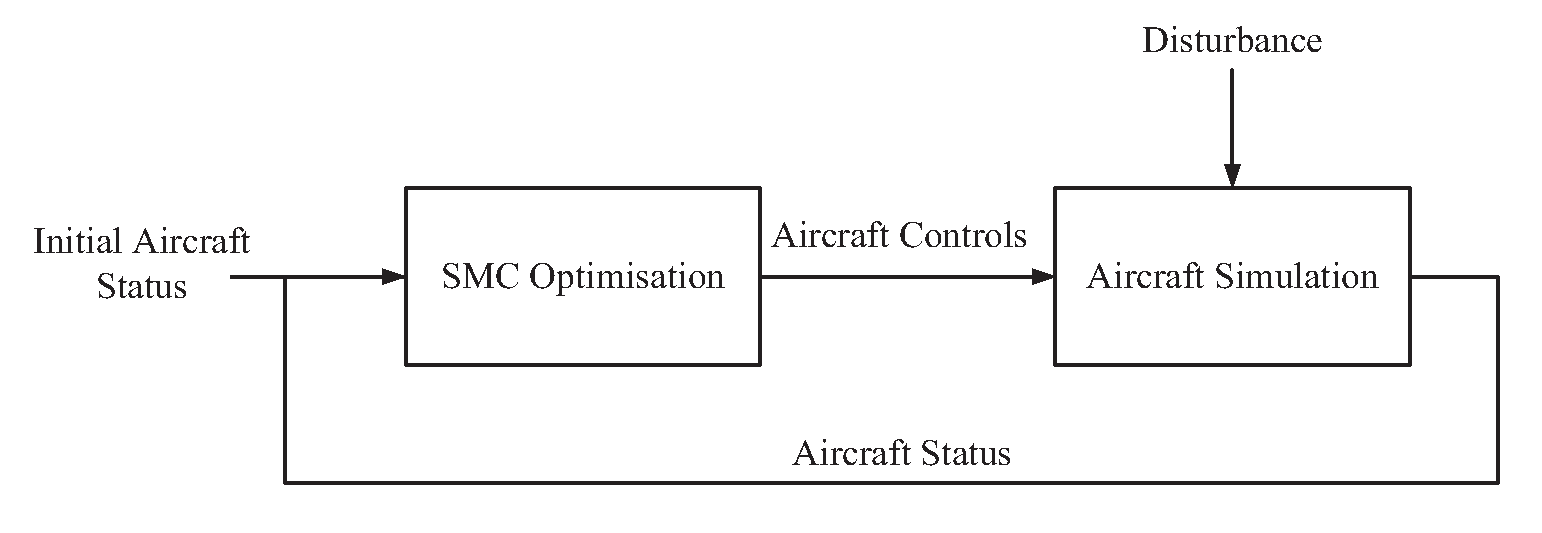
\includegraphics[width=0.75\textwidth]{2_background/figures/smc_mpc}
\end{center}
\caption{An overview of the air traffic control problem.}
\label{fig:smc_mpc}
\end{figure}

%At each sampling instant, a control sequence over a number of future time steps is estimated.
Figure~\ref{fig:atm_model} depicts the model that simulates the dynamic of an aircraft.
The major variables include the aircraft position in 3 dimensional space $(x,y,a)$, true air speed $V$, aircraft mass $m$, heading angle $\chi$, roll angle $\phi$ and pitch angle $\tau$.
The forces applied to the aircraft are its weight $mg$, the engine thrust $T$, and the aerodynamic forces of lift $L$ and drag $D$.
As illustrated in Equation~\ref{eq:atm_c}, $\phi_t$, $\tau_t$ and $T_t$ are control variables which determines the movement of aircraft at time-step $t$.
They are chosen within permitted range and are summerised as a state $s_t$, which is optimised by \gls{smc}.
The state is affected by disturbances from varying wind and atmospheric conditions, therefore, $\phi^{\prime}_t$, $\tau^{\prime}_t$ and $T^{\prime}_t$ represent variables with the effect of disturbances taken into account.
Then the state adjusts the status of aircraft $r_{t}$, which are the position $(x_t, y_t, a_t)$, heading $\chi_t$, speed $V_t$ and mass $m_t$ of the aircraft as described in Equation~\ref{eq:atm_s}.
Table~\ref{tab:atm_variables} summerises the variables used in air traffic management model.
%For more details of the model, see~\cite{eele13cdc}.
%A state is a set of control sequences $\{s_t^{(i),0...H-1}\}^{N_P}_{i=1}$ being picked within a permitted range and applied to the current reference status $r_{t-1}$ to compute the future set of reference statuses $\{r_t^{'{(i),0...H-1}}\}^{N_P}_{i=1}$.
%The variable $H$ is the prediction horizon which means \gls{smc} consider the future $H$ time steps during the optimisation process.

%During importance weighting, a score function evaluates the quality of estimation for each particle, and weights the product of scores over the horizon.
%If any particle violates any constraint, its weight is set to zero
%The first control $s_{t}^0$ in the sequence, is obtained by selecting the best one among $\{s_t^{(i),0...H-1}\}^{N_P}_{i=1}$.
%Then the selected control is committed to form reference $r_t$.

\setcounter{subfigure}{0}
\begin{figure}[t!]
\centering
\subfigure[]{
	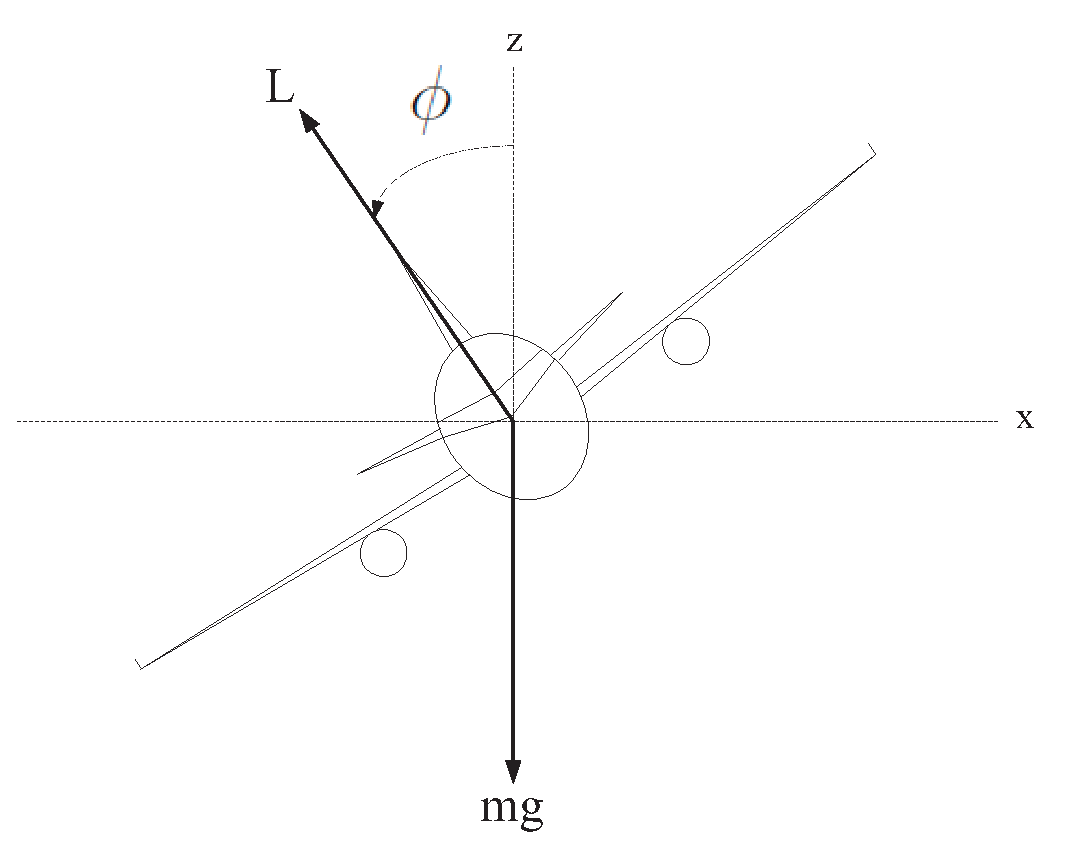
\includegraphics[width=0.32\textwidth]{2_background/figures/atm_model_a}
	\label{fig:atm_model_a}
}
\subfigure[]{
	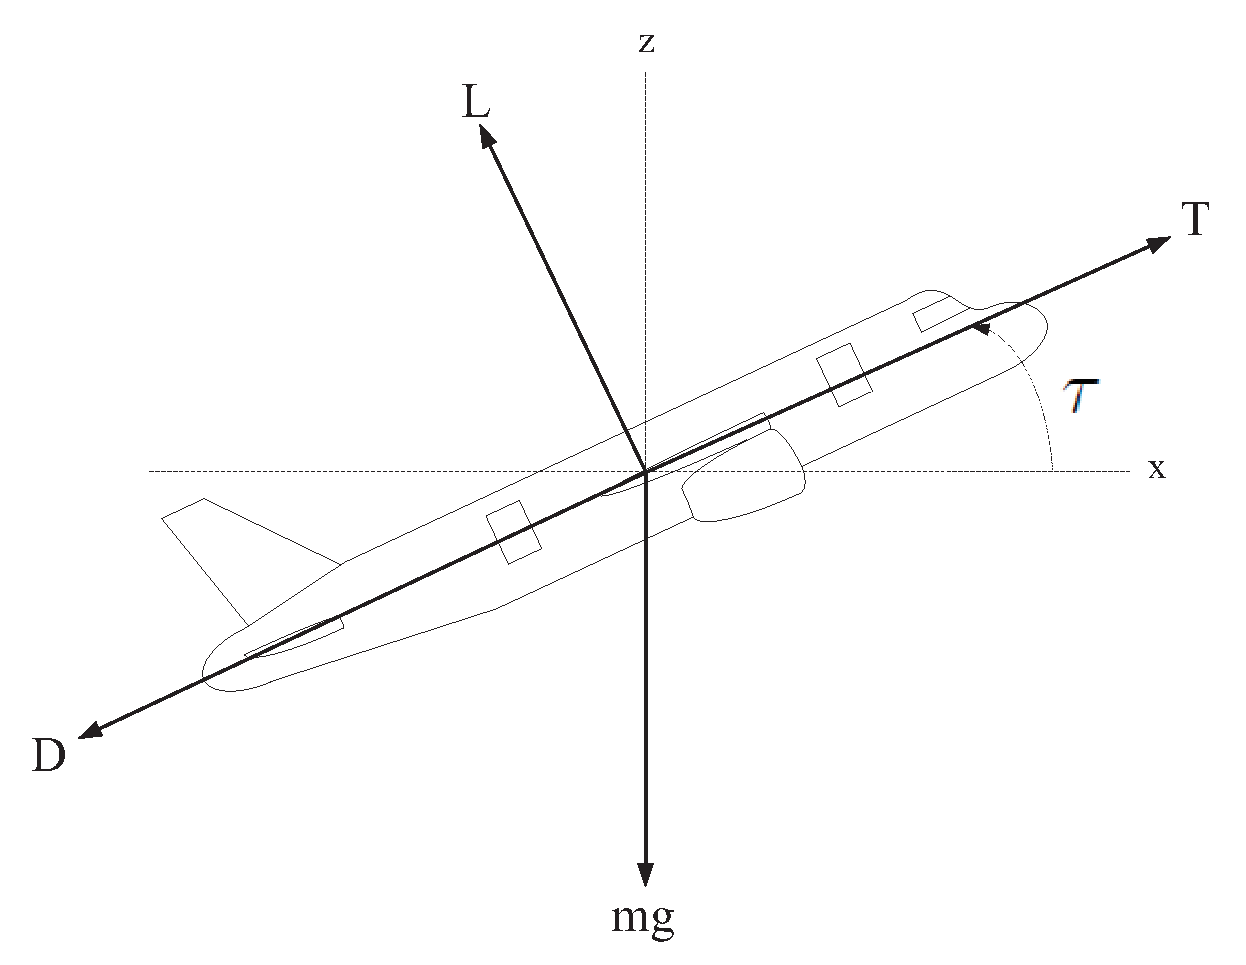
\includegraphics[width=0.32\textwidth]{2_background/figures/atm_model_b}
	\label{fig:atm_model_b}
}
\subfigure[]{
	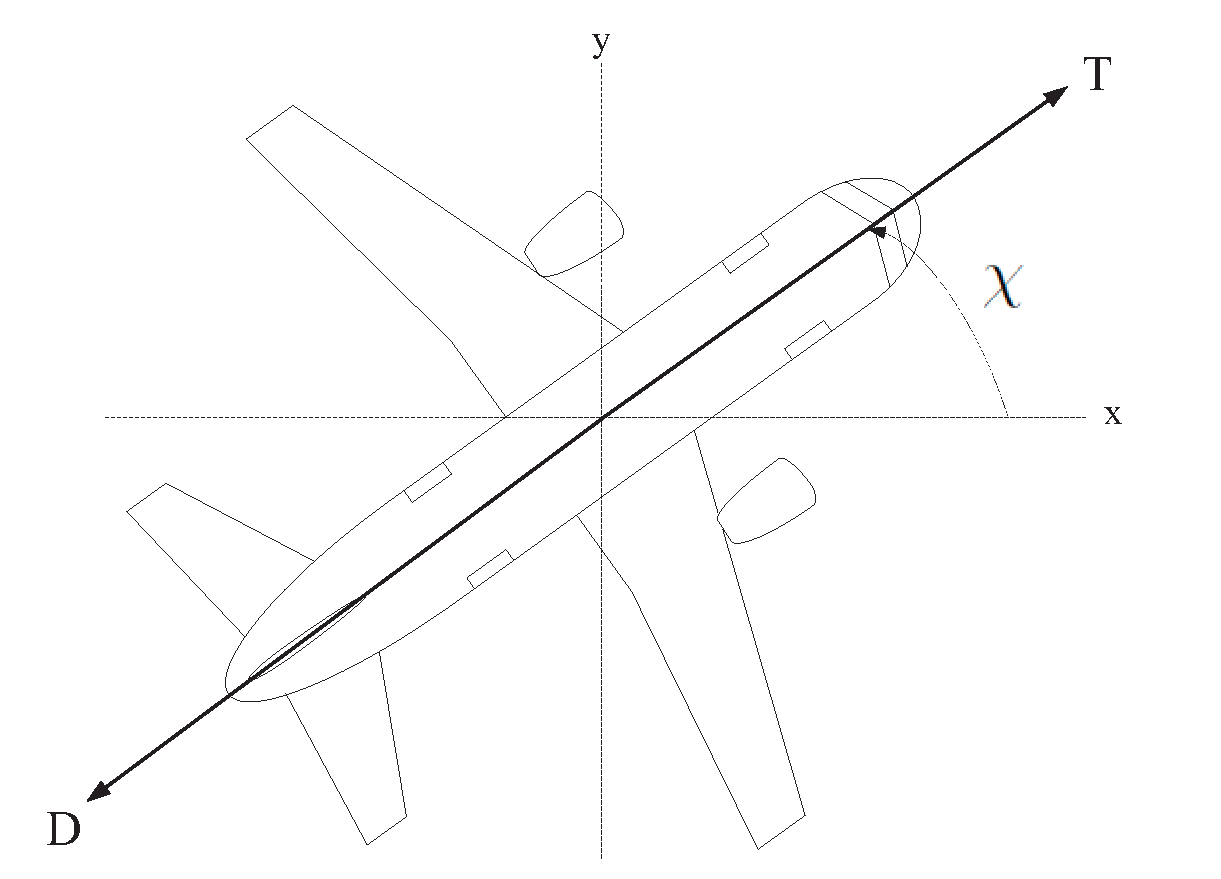
\includegraphics[width=0.32\textwidth]{2_background/figures/atm_model_c}
	\label{fig:atm_model_c}
}
\caption{Aircraft model.}
\label{fig:atm_model}
\end{figure}

\begin{equation}
\begin{aligned}
  \begin{pmatrix}
    s^{\prime(i)}_{t}    \\ 
  \end{pmatrix}
  =
  \begin{pmatrix}
  	\phi^{\prime(i)}_{t} \\
		\tau^{\prime(i)}_{t} \\
		T^{\prime(i)}_{t} \\
  \end{pmatrix}
  =
  \begin{pmatrix}
  	\mathcal{N}(\phi_{t},\sigma_a^2) \\
  	\mathcal{N}(\tau_{t},\sigma_b^2) \\
  	\mathcal{N}(T_{t},\sigma_c^2) \\
  \end{pmatrix}
	\mbox{, }
\end{aligned}
\label{eq:atm_c}
\end{equation}

\begin{equation}
\begin{aligned}
  \begin{pmatrix}
    r^{(i)}_{t}    \\ 
  \end{pmatrix}
  =
  \begin{pmatrix}
    x^{(i)}_{t}    \\ 
    y^{(i)}_{t}    \\ 
    a^{(i)}_{t}    \\ 
    \chi^{(i)}_{t} \\ 
    V^{(i)}_{t}    \\ 
    m^{(i)}_{t}    \\ 
  \end{pmatrix}
  =
  \begin{pmatrix}
    x_{t-1}   + V_{t-1} \cos(\chi_{t-1}) \cos(\tau^{\prime(i)}_{t}) \\
    y_{t-1}   + V_{t-1} \sin(\chi_{t-1}) \cos(\tau^{\prime(i)}_{t}) \\ 
    a_{t-1}   + V_{t-1} \sin(\tau^{\prime(i)}_{t}) \\
    \chi_{t-1} + L \sin(\phi^{\prime(i)}_{t})/(M_{t-1} V_{t-1}) \\
    V_{t-1}   + (\frac{T^{\prime(i)}_{t}-D}{M_{t-1}} - g \sin(\tau^{\prime(i)}_{t})) \\
    m_{t-1}   - \eta T^{\prime(i)}_{t}  \\
  \end{pmatrix}
	\mbox{, }
\end{aligned}
\label{eq:atm_s}
\end{equation}

where $V^{(i)}_{t} \subset [V_{min}, V_{max}]$, $m^{(i)}_{t} \subset [m_{min}, m_{max}]$, $T^{(i)}_{t} \subset [T_{min}, T_{max}]$, $\phi^{(i)}_{t} \subset [\phi_{min}, \phi_{max}]$, $\tau^{(i)}_{t} \subset [\tau_{min}, \tau_{max}]$ are constraints.

\begin{table}
	\setlength{\tabcolsep}{3pt}
	\begin{spacing}{1.0}
	\caption{Variables in air traffic management model.}
	\label{tab:atm_variables}
	\footnotesize
	\centering
	\smallskip
		\begin{tabular}{c|c}
			\hline
			 Variables & Description\\
			\hline
			\hline
			$(x,y,a)$ & Aircraft position in 3 dimensional space \\
			$V$ & True air speed \\
			$m$ & Aircraft mass \\
			$mg$ & Aircraft weight \\
			$\chi$ & Heading angle \\
			$\phi$ & Roll angle \\
			$\tau$ & Pitch angle \\
			$T$ & Engine thrust \\
			$L$ & Lift \\
			$D$ & Drag \\
			\hline
		\end{tabular}
		\end{spacing}
\end{table}

%\subsection{Acceleration of SMC Methods}

%While \gls{smc} has been implemented efficiently on \gls{fpga}s~\cite{chau14trets,chau13acm,happe13,hendeby07}, design productivity remains a challenge.
%Firstly, while different sets of \gls{smc} parameters produce the same accuracy, they have very different computational complexity.
%For example, the performance of \gls{smc} relies on a set of random samples, which are called particles in the following.
%The more complex the problem, the larger the number of particles needed.
%Using excessive numbers of particles unfortunately causes prohibitive run-time without increasing solution accuracy.
%The parameter space spans multiple dimensions and the objective function can be non-convex, making exhaustive optimisation impractical.
%Secondly, customising designs for different \gls{smc} applications requires tremendous effort.

\section{Summary}
\label{sec:bg_summary}

This chapter reviews the architecture and design flow of reconfigurable systems.
Reconfigurable systems provide high flexibility and performance by customising numerous fine-grained resources and implementing massively parallel circuits.
Therefore, reconfigurable hardware are seen as co-processors to offload general-purpose micro-processors, and they are used as accelerators in \gls{hpc}.
When applying reconfigurable technologies to real-time applications, challenges remain in mapping of real-time algorithms to reconfigurable systems.
Apart from performance improvement, the implementations should ensure timeliness, robustness and predictability to support real-time.
The following chapters in this thesis will discuss various approaches to optimise reconfigurable systems for real-time applications, and achieve improvement in terms of computation speed, power consumption and quality of solution.

This chapter mentions the issues of the traditional \gls{fpga} design flow, such as long synthesis time and manual design space analysis.
Academia and industry have been working on \gls{hls} and domain-specific languages to reduce the development effort of reconfigurable systems.
Later in this thesis, we will demonstrate a domain-specific design flow for real-time applications on reconfigurable systems.

%This thesis focuses on optimising reconfigurable systems to accelerate the above mentioned high-performance, real-time applications.
Lastly, this chapter reviews real-time systems and several related applications, which specifically require high-performance.
Subsequent chapters of this thesis will discuss how these applications are accelerated by reconfigurable technologies.
%which relate to the contributions presented in Chapter~\ref{ch:introduction}.
